\chapter{The Evolution of Specialization through Genotypic Polymorphism}
\label{chapter:C2_article2}

\setcounter{secnumdepth}{0}
\setcounter{minitocdepth}{1}
\minitoc[n] % minitoc without title

We now investigate the evolution of division of labour between heterogeneous robots via genotypic polymorphism. Results are presented as a published article in an international conference:

\begin{quote}
  \fullcite{Bernard2016b}
\end{quote}


In the previous Chapter we showed that it could be beneficial to consider the quality of cooperative behaviours in addition to the probability to evolve cooperation. In particular, we revealed that a particular heterogeneous approach, cooperative coevolution, led to the emergence of a more efficient coordination behaviour: leader/follower. This behaviour entails the evolution of task specialisation (or division of labour). Here we focus on the evolution of a leader/follower strategy in a single population of individuals. 

Because in evolutionary robotics cooperation is often evolved among homogeneous robots, this means that in order to achieve division of labour, individuals must be capable to dynamically allocate their roles during their lifetime. In consequence, specialisation often relies on neuronal plasticity or environmental cues. Here we are interested in evolving specialisation without additional mechanisms. This means that we want to achieve division of labour at the level of the population. In consequence, we want to investigate the maintenance of several different genotypes encoding for different roles in a single population, i.e. genotypic polymorphism. In particular, we focus on the impact of selection strategies on evolving genotypic polymorphism.

To that end, we use a simpler foraging task than the one presented in Chapter~\ref{chapter:C2_article1}. Two genetically different individuals are placed in arena where they can collect a single type of targets. This target is more rewarding when collected in a cooperative manner. This means that evolving cooperation is easy (we are not interested in the issue of evolving cooperation here) and that the task if favored by the evolution of efficient coordination strategies. As we showed in the previous Chapter, two different cooperative strategies can evolve in this setting. On the one hand, there is the turner strategy, where both individuals adopt the same behaviour to coordinate. Therefore this is a generalist behaviour. On the other hand, they can also evolve specialist behaviours and adopt a leader/follower strategy. We are interested on studying the evolutionary differences of two selection schemes: (1) a \((\mu + \lambda)\)-ES (elitist) selection strategy and (2) fitness-proportionate selection. We also study the impact of varying population size.

We reveal that specialisation is nearly impossible to evolve under an elitist selection strategy. Indeed, in only one replication under high population size do we observe the presence of specialists in the population at the end of evolution. Surprisingly however, specialists do appear in multiple replications but are never maintained. Even when the population is initially seeded with specialists, similar results are observed. In comparison, while specialists are nearly never evolved under fitness-proportionate selection, they are easily maintained throughout evolution (especially when starting with a population of specialists). We thus reveal that evolving genotypic polymorphism is hindered by the challenge of both evolving and maintaining specialists in the population and that none of these two classical selection schemes are suitable to that end.

We then use computational analyses to have a deeper understanding of the underlying dynamics at play. We show that while specialists are the most efficient, generalists can invade the population because they fare quite well against any other phenotype. In comparison, specialists need to be paired with other specialists of a different type to perform adequatly. Additional analyses show that, under finite population size genetic diversity can be lost from one generation to the other. This can, especially with small population sizes, lead to the disappearance of specialists from the population. We thus highlight two critical properties for the evolution of genotypic polymorphism: (1) protection against the invasion of generalists and (2) maintenance of genotypic diversity. We argue that an algorithm endowed with such properties would enable genotypic polymorphism to be achieved.

\clearpage

\begin{flushleft}
\textbf{\Huge Evolving Specialisation in a Population of Heterogeneous Robots: the Challenge of Bootstrapping and Maintaining Genotypic Polymorphism}
\end{flushleft}


\section{Abstract}
  In this article, we are interested in the evolution of specialisation among a single population of heterogeneous robotic agents in a cooperative foraging task. In particular, we want to compare (1) the emergence and (2) fixation of genotypic polymorphism under two different selection methods: elitist and fitness-proportionate. We show that, while the emergence of specialists is easy under an elitist selection, this method cannot maintain heterogeneous behaviours throughout the whole simulation. In comparison a fitness-proportionate algorithm proves to be inefficient in evolving any cooperative strategy but ensures the conservation of heterogeneity when it is present in the population. We then reveal through additional experiments two key factors for the evolution of heterogenous behaviours in our task: (1) protection of genotypic diversity and (2) efficient selection of partners. We finally demonstrate this assertion and, while our main problem remains unsolved, we provide directions on how it could be successfully approached.


\section{Introduction}
  Task specialisation is a defining characteristic in achieving efficient coordination and is thus considered to be crucial in the evolution of complex cooperative behaviours~\parencite{Eors1995}. The problem of evolving cooperation has been largely studied in evolutionary robotics as it raises interesting persepectives for the design of collective robotics~\parencite{Trianni2007, Hauert2014, Doncieux2015a}. As a consequence, the manner in which robotic agents could evolve specialisation (or division of labour) for a cooperative task represents a compelling challenge in evolutionary robotics. As such, a large body of litterature has already been dedicated to this subject. However, most research focus on the particular case of homogeneous groups of individuals~\parencite{Waibel2009} as is classic in evolutionary robotics. This means that the individuals are forced to rely on phenotypical plasticity~\parencite{Waibel2006, Ferrante2015, Eskridge2015} and/or environmental cues~\parencite{Waibel2006, Goldsby2010} in order to achieve specialisation.

  In this paper, we focus on a slightly different problem: the evolution of a polymorphic population where division of labour is encoded at the genotypic level. More precisely, we want to study the evolution of a population containing two (or more) different types of genotypes. Each of these types of genotype should be able to encode for a different role without requiring the addition of mechanisms for lifetime specialisation. Thus it poses the problem of both \emph{evolving} and \emph{maintaining} genotypic polymorphism in a single population. Here we want to investigate the conditions under which specialised behaviours for a cooperative task can evolve in a single population of heterogeneous individuals. In particular, we are interested in the influence of the selection process in achieving division of labour. 

  We design a 2-robots cooperative foraging task where both a solitary and a cooperative strategies can evolve but where cooperation is highly rewarded. The genotype of each robotic agent is separately chosen in the population and the individuals therefore form an heterogeneous group. This task is greatly favored by the evolution of efficient coordination strategies. In particular, our previous work on a similar task~\parencite{Bernard2015} showed that two types of cooperative strategy could evolve: one where both individuals adopt homogeneous behaviours (generalists) and the other one where they adopt a leader/follower strategy (specialists). Moreover, it was shown that the latter could only emerge between heterogeneous individuals. As it is also the more efficient behaviour, we study the conditions for its emergence. The evolutionary dynamics of two popular selection methods are studied: (1) an elitist \((\mu + \lambda)\) evolution strategy and (2) fitness-proportionate selection. Fitness-proportionate in particular is interesting with regards to genotypic polymorphism as it is known to allow the evolution of frequency-dependent selection~\parencite{Altenberg1991}.

  In the next Section, we introduce the experimental setup. Then we present the two types of cooperative strategies that can evolve. Next, we investigate whether any of the selection methods could evolve heterogeneous behaviours. In particular, we study for both schemes the evolutionary outcomes depending on whether the population is initially constituted of random individuals or seeded with pre-evolved efficient specialists. Then we present the results of computational analyses in order to reveal and understand more deeply the mechanisms at play. In a final experiment, we reveal key mechanisms which could be investigated to solve this problem. Finally we discuss our findings and shed light on interesting perspectives for future work.




\section{Methods}
\label{sec:methods}
  We evaluate two robotic agents in a $800$ by $800$ units square arena devoid of any obstacles except for the foraging targets. At the beginning of a simulation, $18$ targets are randomly positioned in the environment. While the agents may move freely in the arena, the targets' positions are fixed. For a target to be collected, any agent needs to stay in contact with it for a specified amount of time ($800$ simulation steps). The target is removed after this duration and put back at another random position so that the number of targets is kept the same throughout a simulation. We consider that cooperative foraging happens if both individuals are in contact of the target when it is removed. When an agent collects a target, it is rewarded \textbf{50} if this target has been foraged in a solitary manner or \textbf{250} if both agents have cooperated to collect it.
  
  \begin{table}[h]
    \center{
      \begin{tabular}{|l|c|}
        \hline
        \textbf{Foraging} & \textbf{Reward} \\
        \hline
        \hline
        \textbf{Solitary} & 50 \\
        \textbf{Cooperatively} & 250 \\
        \hline
      \end{tabular}
    }
    \caption{\textbf{Rewards for the foraging of targets.}
    Rewards depend on whether the targers were collected in a solitary or cooperative fashion.}
    \label{tab:Rewards}
  \end{table}

  Each agent is circular-shaped with a diameter of $20$ units and possesses a collection of different sensory inputs. The first type of inputs is a $90$ degrees front camera and is composed of $12$ rays, each one indicating the type and distance to the nearest object (either another agent or a target). The other type of inputs are $12$ proximity sensors evenly distributed around the agent's body. With a range of twice the agent's diameter, each proximity sensor outputs the proximity of the nearest obstacle in its range.

  Both agents begin the simulation next to each other at the same end of the arena and can move according to the outputs of their neural network. This neural network is a fully connected multi-layer perceptron with one hidden layer. The inputs of the neural network are comprised of all the sensory information of the agent, i.e. $36$ input neurons for the camera ($3$ inputs for each ray) and $12$ for the proximity sensors. A final input neuron whose value is always $1$ is used as a bias neuron. This amounts the total number of input neurons to $49$. The hidden layer is constituted of $8$ neurons while the $2$ neurons of the output layer return the speed of the agent's wheels. A sigmoid is used as the activation function of each neuron. Finally, the topology of the network is kept constant during the experiments.

  The population of individuals is evolved thanks to a classical evolutionary algorithm. The genotype of each individual is constituted of a collection of the $410$ real-valued connection weights of the neural network. At each generation of the algorithm, every individual is evaluated by being successively paired with another individual randomly chosen in the population $5$ times. Each pair interacts in the setting presented before during $20000$ simulation steps which we call a \emph{trial}. We perform $5$ trials for each pair of individuals in order to decrease the impact of the targets' random positions on the individuals' performance. The fitness score of an individual is computed as the average reward per trial.

  The population for the next generation is created according to two different selection schemes :

  \begin{itemize}
    \item{\textbf{\((\mu + \lambda)\) elitist selection:} the population of the next generation is constituted of the $\mu$ best individuals from this generation and $\lambda$ offsprings sampled from the best individuals.}
    \item{\textbf{Fitness-proportionate:} offsprings are randomly sampled from the current generation to constitute the population of the next generation. The probability to sample a particular parent is proportional to this parent's fitness score.}
  \end{itemize}

  Regardless of the selection method used, every offspring is a mutated clone of its parent and no recombination is used in our algorithm. The probability for each gene to mutate is \(5 \times 10^{-3}\) and mutations are sampled according to a gaussian operator with a standard deviation of \(2 \times 10^{-2}\). Finally, experiments were conducted with the robotic 2D simulator of SFERESv2~\parencite{Mouret2010}, a framework for evolutionary computation. You can find the source code for the experiments available for download at http://pages.isir.upmc.fr/\textasciitilde bredeche/Experiments/ALIFE2016-specialisation.tgz.
    

\section{Behaviours of Specialists in a Cooperative Foraging Task}
\label{sec:efficiency}
  We showed in a previous article~\parencite{Bernard2015} that two cooperative strategies could evolve in this particular task: \emph{turning} (between two \emph{turners}) and \emph{leader/follower} (between a \emph{leader} and a \emph{follower}). Both of these strategies achieve cooperative foraging but with varied efficiency.

  \begin{figure}[ht]
    \centerfloat
      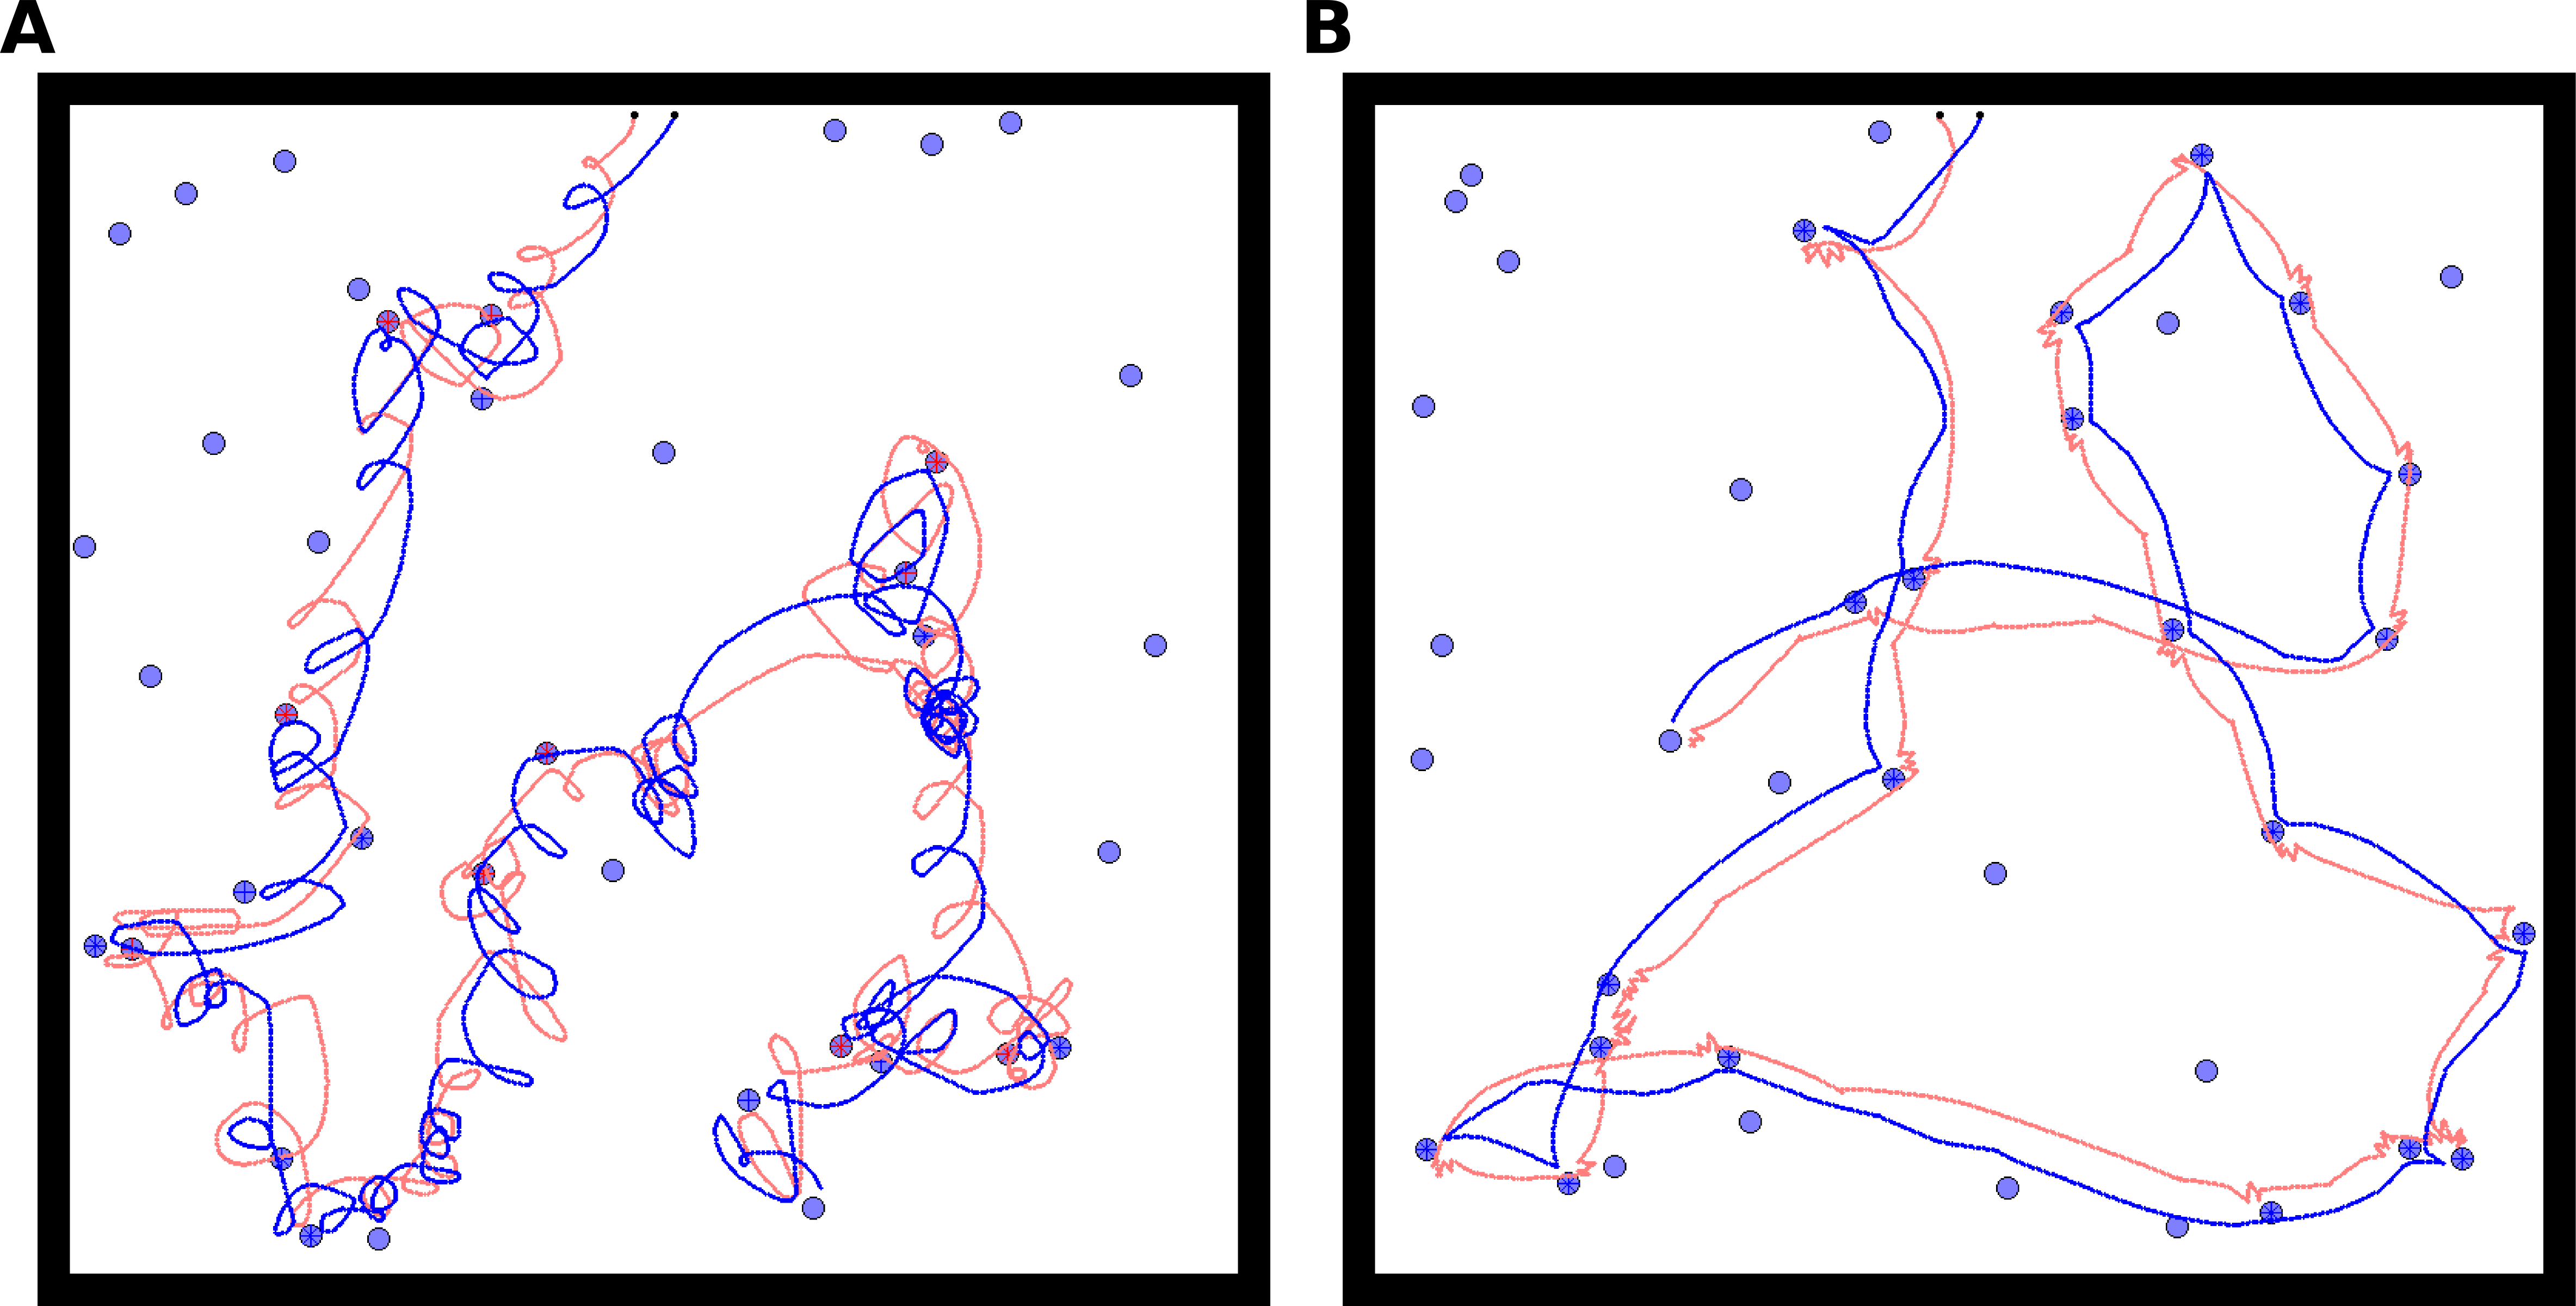
\includegraphics[scale=0.7]{fig/ArticleRob2/figBehaviours.png}
    \caption{\textbf{Snapshots of the simulation after an entire trial in the foraging task.} The path of each robotic agent from their initial positions (black dots) is represented in red and blue. The blue discs represent the 18 targets in the environment. When a target is foraged by the two agents, a red cross (resp. blue) is drawn on the target if the red agent (resp. blue) arrived on it first. Each snapshot corresponds to a trial where agents adopted a different strategy: {\em (A)}~turning or {\em (B)}~leader/follower.}
    \label{fig:behaviorTraces}
  \end{figure}

  In the turning strategy, both individuals turn around one another so that they can keep the other individual in their line of sight and stay close to it (see Figure \ref{fig:behaviorTraces}(A)). At the same time, the two individuals try to get closer to a target. This way, as soon as one of the two individuals is in contact with a target, the other individual can join it so the target may be collected cooperatively. Consequently, both individuals adopt a similar behaviour in this strategy and can be described as generalists.

  In the leader/follower strategy, the individuals specialise in two roles: a leader and a follower. The leader always gets on the target first and checks rarely for its partner. In comparison, the follower tries to keep its leader in view during the entirety of the simulation so that it can get on the same target (see Figure \ref{fig:behaviorTraces}(B)). Consequently, we observe the expression of two clearly heterogeneous behaviours which implies that both individuals are specialists. More importantly we also showed that, given our agents' capabilities, each phenotype needed to be encoded by a different genotype for specialisation to happen.

  \begin{figure}[ht]
    \centerfloat
      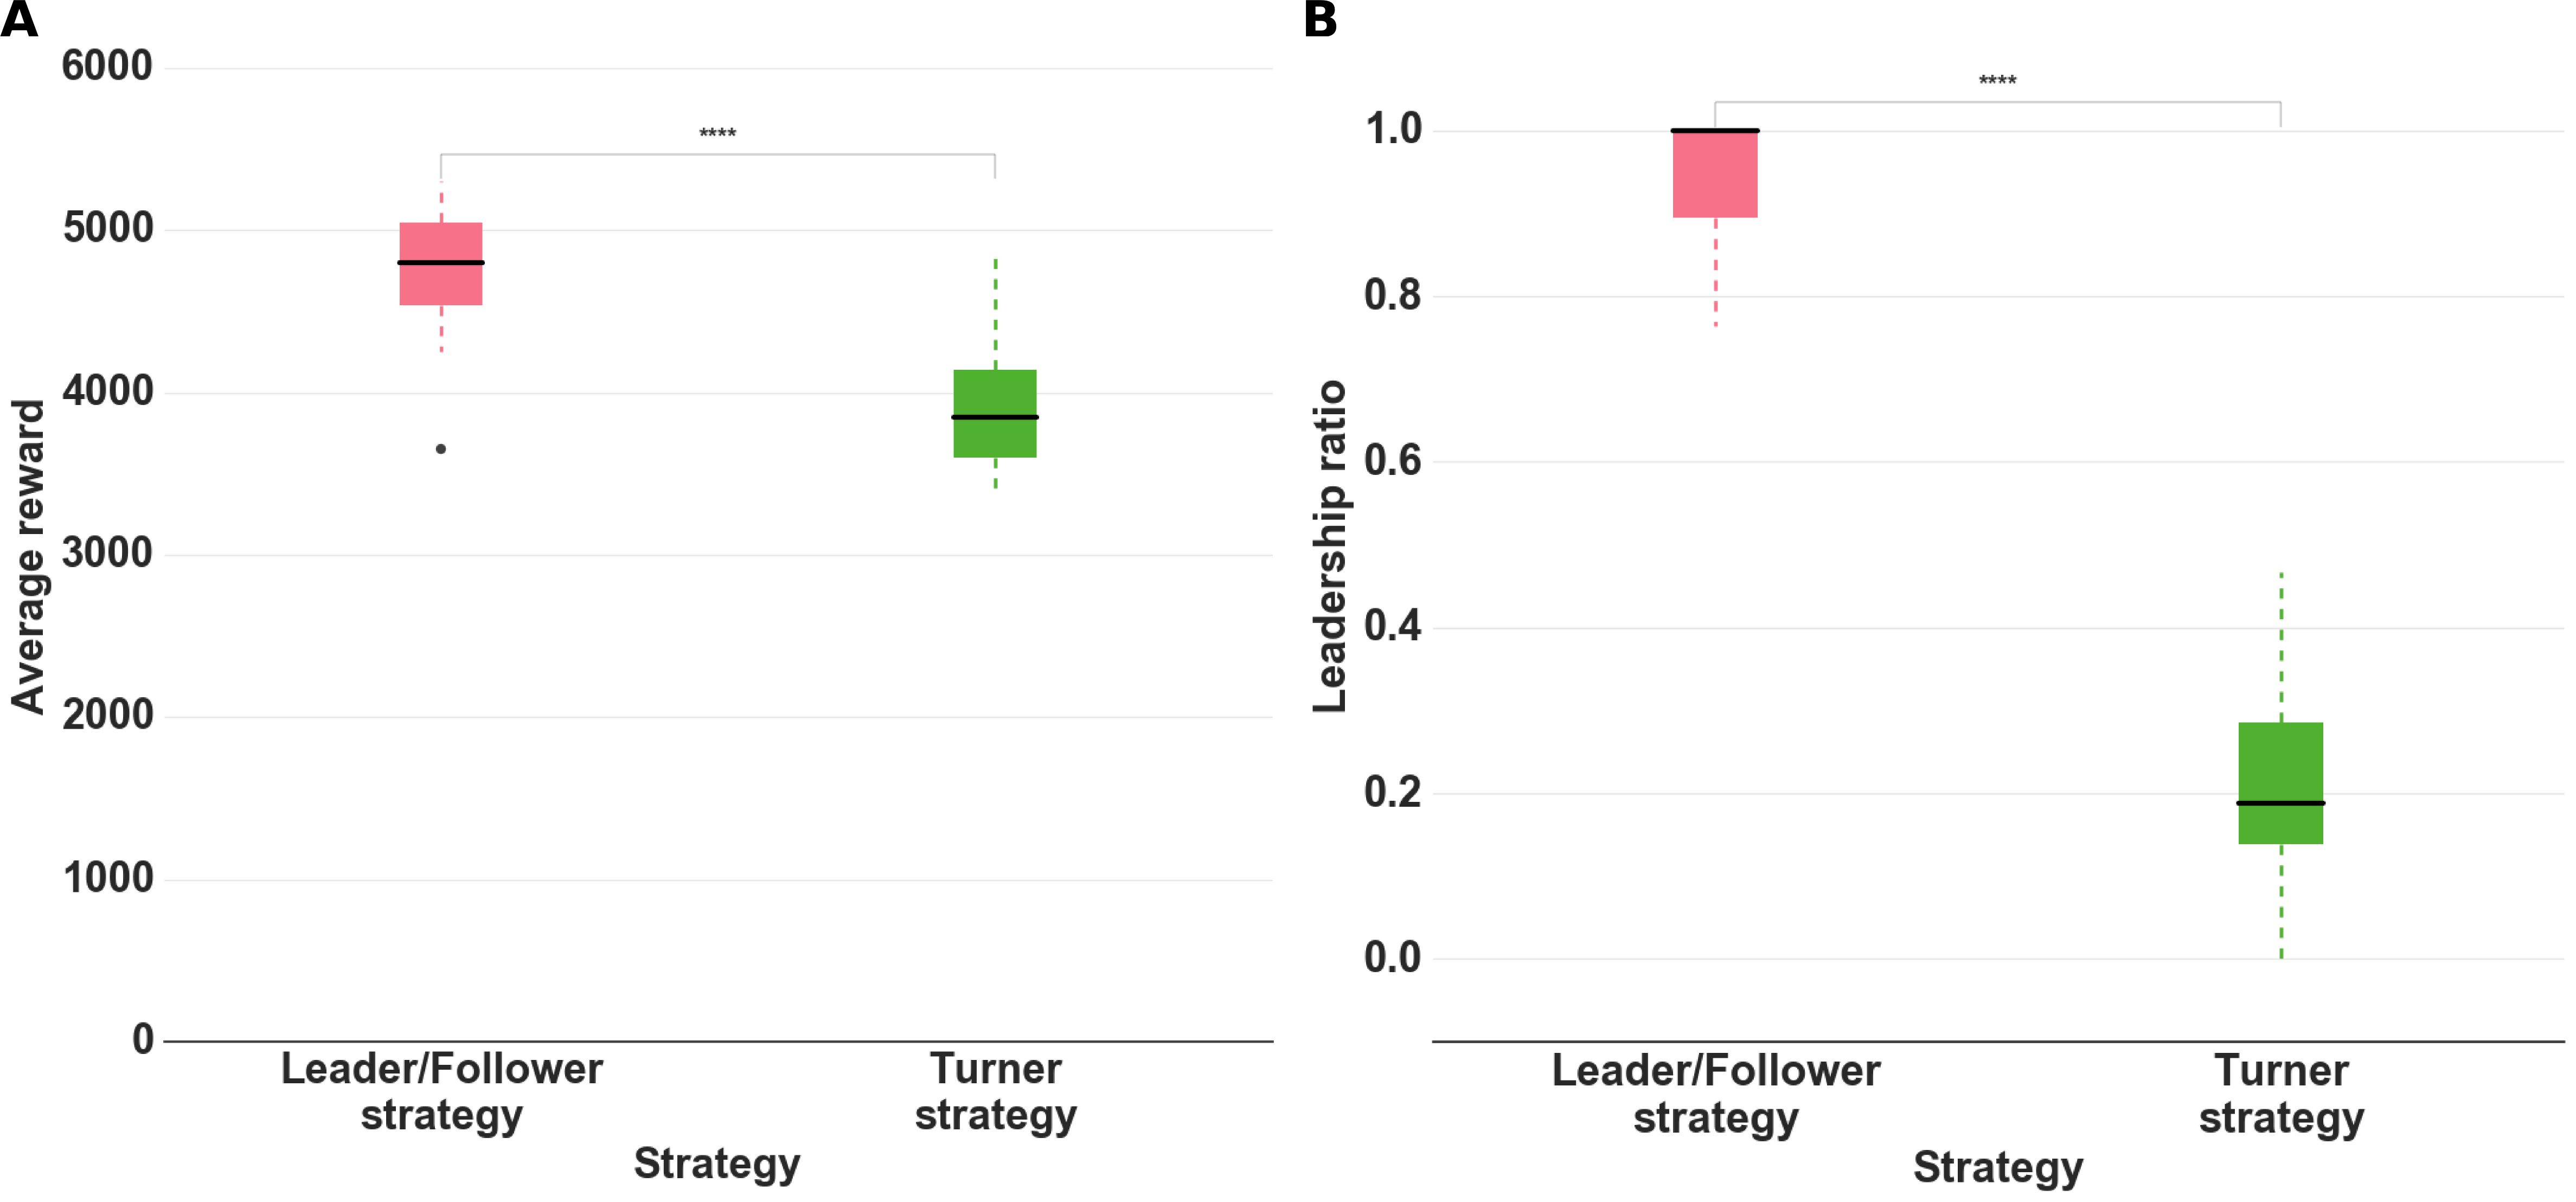
\includegraphics[scale=0.9]{fig/ArticleRob2/figEffAndLead.png}
    \caption{\textbf{Average reward and leadership proportion with a leader/follower or turning strategy} Boxplots of {\em (A)}~the average reward and {\em (B)}~the leadership proportion over $20$ independent trials for the leader/follower and turning strategies. The leadership ratio of an individual represents the propensity for one individual among the pair to arrive first more often than its partner on a target collected in a cooperative fashion. The position of each target at the beginning of each trial was randomized.}
    \label{fig:EfficiencyAndLeadership}
  \end{figure}

  Figure~\ref{fig:EfficiencyAndLeadership}(A) shows the efficiency of each strategy, defined as the average reward obtained by the two individuals during a simulation over $20$ independent trials (with randomized targets' positions for each trial). We can see that, as expected, the leader/follower strategy achieves a significantly higher efficiency (Mann-Whitney U-test on the average reward over $20$ trials, {\em p}-value $< 0.0001$). This difference in efficiency is directly correlated to a highly significant difference in the proportion of leadership as shown in Figure~\ref{fig:EfficiencyAndLeadership}(B) (Mann-Whitney U-test on the leadership proportion over $20$ trials, {\em p}-value $< 0.0001$). We compute this proportion by looking at the propensity for one of the two individuals to arrive first more often on a target foraged cooperatively (i.e. the emergence of a leader).



\section{Evolving Heterogeneous Behaviours with an Elitist Selection}
\label{sec:elitistEvolution}
  \subsection{Bootstrapping leader/follower strategies}
    In this first experiment, we are interested in the emergence of a leader/follower strategy when starting with a population of random individuals under an \((\mu + \lambda)\) elitist selection. In order to investigate the influence of population size, we tested three different sizes \(N\): $20$, $40$ and $100$. For each population size, we conducted $11$ independent runs, each one lasting $90000$ evaluations. For each population size \(N\), we defined \(\mu\) (i.e. the number of parents) and \(\lambda\) (i.e. the number of offsprings) as \(\frac{N}{2}\). For example, when population size was $100$, $50$ individuals were kept from the previous generation and used to create $50$ mutated offsprings.

    \begin{table}[ht]
      \center{
        \begin{tabular}{|l|c|c|c|c|}
          \hline
          \textbf{Pop.} & \textbf{\# L/F} & \textbf{\# Turning} & \textbf{\# NC} & \textbf{Total}\\ 
          \textbf{size} & \textbf{Strat.} & \textbf{Strat.} & \textbf{Strat.} & \\ 
          \hline
          \hline
          \textbf{20} & 0 & 11 & 0 & \textbf{11}\\
          \textbf{40} & 0 & 11 & 0 & \textbf{11}\\
          \textbf{100} & 1 & 10 & 0 & \textbf{11}\\
          \hline
        \end{tabular}
      }
      \caption{\textbf{Strategies evolved by the best individuals under elitist selection with an initially random population.} Repartition of the different strategies adopted by the best individuals at the last evaluation in each of the replicates for different population sizes \(N\). We indicate in each cell the number of simulations where a particular strategy evolved. Populations were evolved under an \((\mu + \lambda)\) elitist selection, with \(\mu = \frac{N}{2}\) and \(\lambda = \frac{N}{2}\). Individuals' genotype values were intially random. In the table "L/F" stands for leader/follower and "NC" for "Non-Cooperative".}
      \label{tab:elitistScratchStrategies}
    \end{table}

    Table~\ref{tab:elitistScratchStrategies} shows the repartition of the best individuals' strategies at the last generation of evolution for each population size. We consider a behaviour to be cooperative when more than 50\% of the total number of targets collected are foraged cooperatively. First, we observe that in every replicate individuals always end up evolving a cooperative strategy. We also see that evolving a leader/follower strategy is difficult as specialists evolve in only $1$ run (out of $33$) and when the population size is $100$. These results suggest that it is nearly impossible to evolve such heterogeneous behaviours with this setting.

    \begin{figure}[ht]
      \centering
        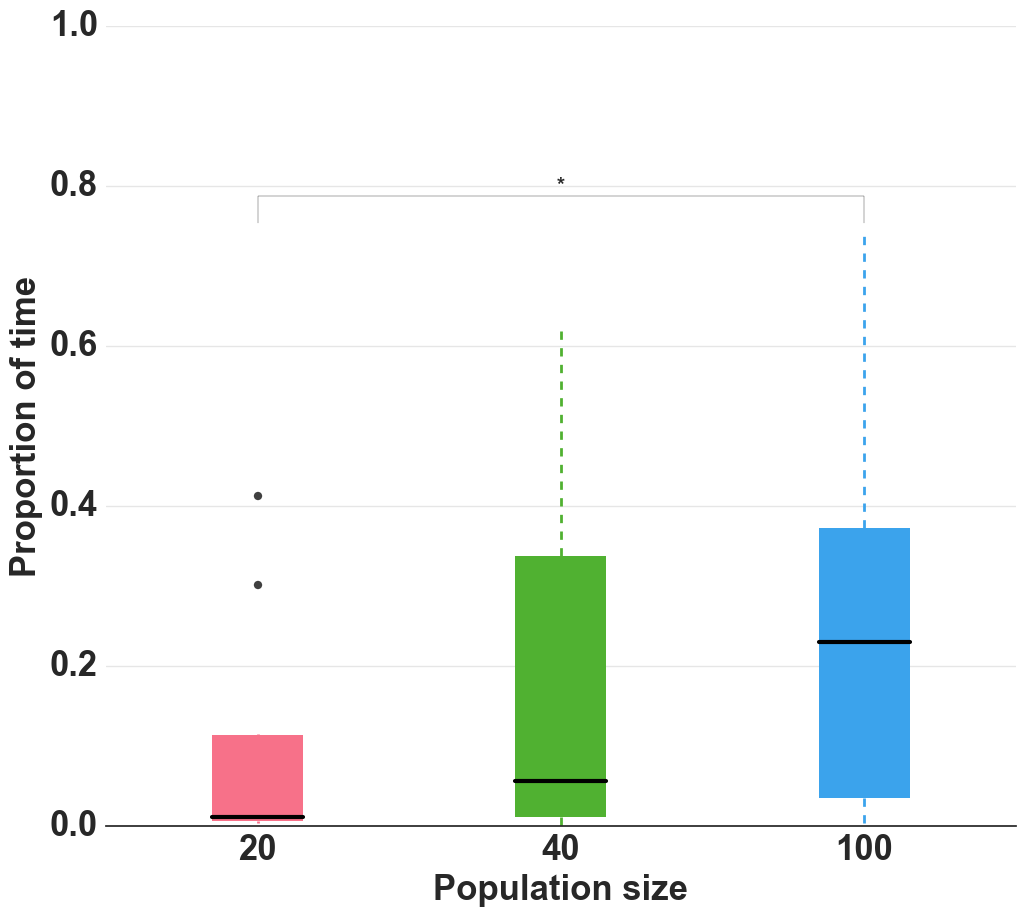
\includegraphics[scale=0.35]{fig/ArticleRob2/boxplotLeadershipTime.png}
        \caption{\textbf{Proportion of time with a leader/follower strategy.} Boxplots of the number of generations where the best individual in each replicate adopted a leader/follower strategy out of the total number of generations. We consider that the best individual adopted a leader/follower strategy when its leadership ratio was over a threshold value of $0.6$.}
      \label{fig:leadershipTime}
    \end{figure}

    However, when looking at the whole evolutionary history we can reveal additional information about the evolution of specialists. We show in Figure~\ref{fig:leadershipTime} the proportion of evolutionary time when the best individual of each run adopted a leader/follower strategy. This value is computed as the ratio of the number of generations when the leadership ratio was high enough (over a threshold value of $0.6$) out of the total number of generations. We observe that even if the best individuals end up adopting a generalist strategy, this was not the case during the entirety of the evolution. In particular, there is a significant increase (Mann-Whitney, {\em p}-value $< 0.05$) in the number of generations where the best individual showed a leader/follower strategy when population size was $100$ compared to a population size of $20$. Therefore this implies that it is possible to evolve specialists but their stability in the population over time is nearly impossible to achieve.


  \subsection{Maintaining heterogeneity in a population seeded with specialists}
    In order to investigate the lack of stability of genotypic polymorphism under elitist selection, we design another experiment. We separately evolve a population of efficient \emph{leader individuals} and \emph{follower individuals} beforehand. We then replace the worst individuals w.r.t. fitness score in the population of leaders by a certain amount of followers. Our goal is to study if artificially constructing such population could result in the invasion and fixation of a stable leader/follower strategy.

    The number of followers initially inserted in the population was varied according to two different settings: (1) we add only one follower or (2) we add an amount of followers equal to half of the population. Experiments were replicated $11$ times during $90000$ evaluations with population size of $40$ and $100$.

    \begin{table}[ht]
      \center{
        \begin{tabular}{|l|r|c|c|c|c|}
          \hline
          \textbf{Pop.} & \textbf{Followers} & \textbf{\# L/F} & \textbf{\# Turning} & \textbf{\# NC} & \textbf{Total}\\ 
          \textbf{size} & \textbf{added} & \textbf{Strat.} & \textbf{Strat.} & \textbf{Strat.} & \\ 
          \hline
          \hline
          \textbf{40} & \textit{1} & 0 & 11 & 0 & \textbf{11}\\
          \textbf{40} & \textit{20} & 0 & 11 & 0 & \textbf{11}\\
          \textbf{100} & \textit{1} & 1 & 10 & 0 & \textbf{11}\\
          \textbf{100} & \textit{50} & 2 & 9 & 0 & \textbf{11}\\
          \hline
        \end{tabular}
      }
      \caption{\textbf{Strategies evolved by the best individuals under elitist selection when adding followers.} Repartition of the different strategies adopted by the best individuals at last evaluation in each of the replicates for different population sizes \(N\). We indicate in each cell the number of simulations where a particular strategy evolved. Populations were evolved under a \((\mu + \lambda)\) elitist selection, with \(\mu = \frac{N}{2}\) and \(\lambda = \frac{N}{2}\). The population was initially seeded with a population of leaders in which we added a specific amount of followers. In the table "L/F" stands for leader/follower and "NC" for "Non-Cooperative".}
      \label{tab:elitistInvasionStrategies}
    \end{table}


    We show (Table~\ref{tab:elitistScratchStrategies}) no significant differences in comparison to simulations with a population constituted of initially random individuals w.r.t. the number of simulations where a leader/follower strategy evolved. These results suggest that even when purposely adding specialists, their stability in the population is still very hard to achieve. This implies that whether the behaviours are evolved from random genotypes or bootstrapped with efficient individuals is not as important as maintaining heterogeneity in the population. In particular, in only one replicate among the $3$ runs where a leader/strategy was eventually adopted (out of $44$) did the specialists initially added were maintained. In the $2$ other runs we observe multiple emergences and disappearances of specialists throughout evolution. 


\section{Evolution Under a Fitness-Proportionate Selection}
\label{sec:fitpropEvolution}
  In this next experiment we want to investigate the evolution of heterogeneous behaviours when using a fitness-proportionate selection. As fitness-proportionate is known to allow frequency-dependent selection, we hypothesize that it may facilitate the evolution of specialists.

  \subsection{Bootstrapping leader/follower strategies}
    Similarly to the elitist selection, we replicated our experiments in $11$ independent runs during $90000$ evaluations. Likewise, population sizes were $20$, $40$ and $100$. 
    
    \begin{table}[ht]
      \center{
        \begin{tabular}{|l|c|c|c|c|}
          \hline
          \textbf{Pop.} & \textbf{\# L/F} & \textbf{\# Turning} & \textbf{\# NC} & \textbf{Total}\\ 
          \textbf{size} & \textbf{Strat.} & \textbf{Strat.} & \textbf{Strat.} & \\ 
          \hline
          \hline
          \textbf{20} & 0 & 1 & 10 & \textbf{11}\\
          \textbf{40} & 0 & 1 & 10 & \textbf{11}\\
          \textbf{100} & 1 & 2 & 8 & \textbf{11}\\
          \hline
        \end{tabular}
      }
      \caption{\textbf{Strategies evolved by the best individuals under fitness-proportionate selection with an initially random population.} Repartition of the different strategies adopted by the best individuals at the last evaluation in each of the replicates for different population sizes. We indicate in each cell the number of simulations where a particular strategy evolved. Populations were evolved under a fitness-proportionate selection. Individuals' genotype values were initially random. In the table "L/F" stands for leader/follower and "NC" for "Non-Cooperative".}
      \label{tab:fitpropScratchStrategies}
    \end{table}

    We show in Table~\ref{tab:fitpropScratchStrategies} that results are highly different when using such selection scheme. In particular, the fitness-proportionate selection performed poorly w.r.t. evolving cooperative strategies. For each population size, no cooperative strategy evolved at all in the vast majority of replicates. However in one particular run we do observe the emergence and fixation of specialists. This is similar to what was observed under elitist selection w.r.t. evolving specialists.

    Yet a closer look at the dynamics of evolution under a fitness-proportionate selection yields interesting results. In particular, there is not much variation in the strategy adopted by the best individuals throughout evolution. This is consistent with the fact that the bootstrap of a cooperative strategy was not observed in most of the replicates: fitness-proportionate is not efficient in evolving any cooperative behaviour. In consequence, there is not much variation in the proportion of individuals adopting a leader/follower strategy during evolution. As a matter of fact, we observe that in the only replicate where there was genotypic polymorphism at the end of the simulation, specialists were already present at the random initialisation of the population and did not evolve through mutation. This is very different with the elitist selection where we observe multiple emergences of specialists (even briefly) during evolution in many different runs.

  \subsection{Maintaining heterogeneity in a population seeded with specialists}
    \begin{table}[ht]
      \center{
        \begin{tabular}{|l|r|c|c|c|c|}
          \hline
          \textbf{Pop.} & \textbf{Followers} & \textbf{\# L/F} & \textbf{\# Turning} & \textbf{\# NC} & \textbf{Total}\\ 
          \textbf{size} & \textbf{added} & \textbf{Strat.} & \textbf{Strat.} & \textbf{Strat.} & \\ 
          \hline
          \hline
          \textbf{40} & \textit{1} & 7 & 0 & 4 & \textbf{11}\\
          \textbf{40} & \textit{20} & 8 & 0 & 3 & \textbf{11}\\
          \textbf{100} & \textit{1} & 10 & 0 & 1 & \textbf{11}\\
          \textbf{100} & \textit{50} & 10 & 0 & 1 & \textbf{11}\\
          \hline
        \end{tabular}
      }
      \caption{\textbf{Strategies evolved by the best individuals under fitness-proportionate selection when adding followers.} Repartition of the different strategies adopted by the best individuals at the last evaluation in each of the replicates for different population sizes \(N\). We indicate in each cell the number of simulations where a particular strategy evolved. Populations were evolved under a fitness-proportionate selection. The population was initially seeded with a population of leaders in which we added a specific amount of followers. In the table "L/F" stands for leader/follower and "NC" for "Non-Cooperative".}
      \label{tab:fitpropInvasionStrategies}
    \end{table}

    As expected from previous results, fitness-proportionate performs well in terms of stability of heterogeneous behaviours. We show in Table~\ref{tab:fitpropInvasionStrategies} that in the majority of replicates the best individuals adopt a leader/follower strategy at the end of the simulations. This is particularly true when population size is high enough ($100$). A major difference with the elitist selection is that in all replicates where a leader/follower strategy was observed at the end of the run, the specialists were maintained from the start throughout evolutionary time. These results suggest that, although not efficient at bootstrapping cooperative behaviours, fitness-proportionate performs well w.r.t. the stability of genotypic heterogeneity. Furthermore, we can hypothesize that this selection scheme is good at maintaining heterogeneity specifically because it largely fails (under our choice of parameters) at bootstrapping any cooperative strategy.


\section{Computational Analyses of Population Dynamics}
  In this present section, our goal is to understand more deeply the dynamics at play which allow the invasion of suboptimal generalists even when efficient specialists are present. To that end we run computational analyses based on the expected fitness of each of the three phenotypes. Table~\ref{tab:payoffMatrix} shows the average payoff of pair-wise simulations between each type of phenotypes. We consider the payoffs for both phenotypes in each pair to be identical as no significant differences were observed between their payoffs.

  \begin{table}[h]
    \center{
      \begin{tabular}{|c|c|c|c|}
        \hline
        \textbf{Phenotype} & \textbf{Leader} & \textbf{Follower} & \textbf{Turner} \\
        \hline
        \hline
        \textbf{Leader} & 1265 & 5000 & 3480 \\
        \textbf{Follower} & 5000 & 100 & 2750 \\
        \textbf{Turner} & 3480 & 2750 & 2755 \\
        \hline
      \end{tabular}
    }
    \caption{\textbf{Payoff matrix for pair-wise simulations of each phenotype.} Average payoffs of each phenotype against every phenotype in a pair-wise simulation. Each pair was evaluated $10$ times in order to decrease the stochastic effects of the initial conditions (i.e. random positions of the targets).}
    \label{tab:payoffMatrix}
  \end{table}

  Several observations can be made directly from these results. First, we can confirm that the leader/follower strategy displayed by a (\emph{leader}, \emph{follower}) pair is clearly the best strategy. However each one of these two phenotypes performs very poorly against itself with the worst payoff obtained by a pair constituted of two \emph{followers}. Secondly, \emph{turner} individuals perform also very well against \emph{leaders}. Last, there is no significant differences w.r.t. payoffs when a \emph{turner} is paired with a \emph{follower} or another \emph{turner}. These last two points hint at a shared lineage between \emph{followers} and \emph{turners}. 

  Indeed analyses of the genotypes' histories in our previous experiments reveal that \emph{turner} individuals in fact descend from \emph{follower} individuals. This means that they act as \emph{followers} when interacting with \emph{leaders} but are not as efficient. However they are a lot more efficient than \emph{followers} when paired with individuals of the same phenotype (or \emph{followers}).

  % TODO: Virer le paragraphe précédent ? (notamment pour faire un peu de place)

  From this payoff matrix, we run computational analyses to model the gradient of phenotypes' repartition in an infinite population. The fitness \(W\) of a particular phenotype \(i\) is computed as follows:

  \[
    W_{i} = \sum_{j=1}^{M} P(ij)*F(j)
  \]

  with \(j\) the phenotype it is paired with, \(M\) the number of different phenotypes ($3$), \(P(ij)\) the payoff of phenotype \(i\) against \(j\) and \(F(j)\) the proportion of phenotype \(j\) in the population. From this fitness, we can deduce the variation of phenotypes repartition by updating the proportion \(F\) of each phenotype \(i\): 

  \[
    F_{i} = F_{i}*\frac{W_{i}}{\sum_{j=1}^{M} W_{j}}
  \]

  We show in Figure~\ref{fig:ternary}(A) a vector field of this gradient. We can see that there actually exists an equilibrium between the three phenotypes (marked by the a dot at the crossing between the the dotted lines). This implies that even though the \emph{turner} strategy is not the more efficient one, it is still expected that this phenotype can invade and coexist with the two other phenotypes.

  We can hypothesize that we could not observe this equilibrium in our robotic simulations because of the stochastic effects arising from selection in a finite population. In order to study this hypothesis we ran additional computational simulations based on the same payoff matrix. The initial population is entirely composed of \emph{leaders} and the selection method is an elitist (\(\frac{N}{2}\)+\(\frac{N}{2}\)) evolution strategy where \(N\) is the population size. Every $10$ generations, each offspring has a probability of \(1*10^{-2}\) to mutate into any of the two other phenotypes.

  \begin{figure}[ht]
    \centerfloat
      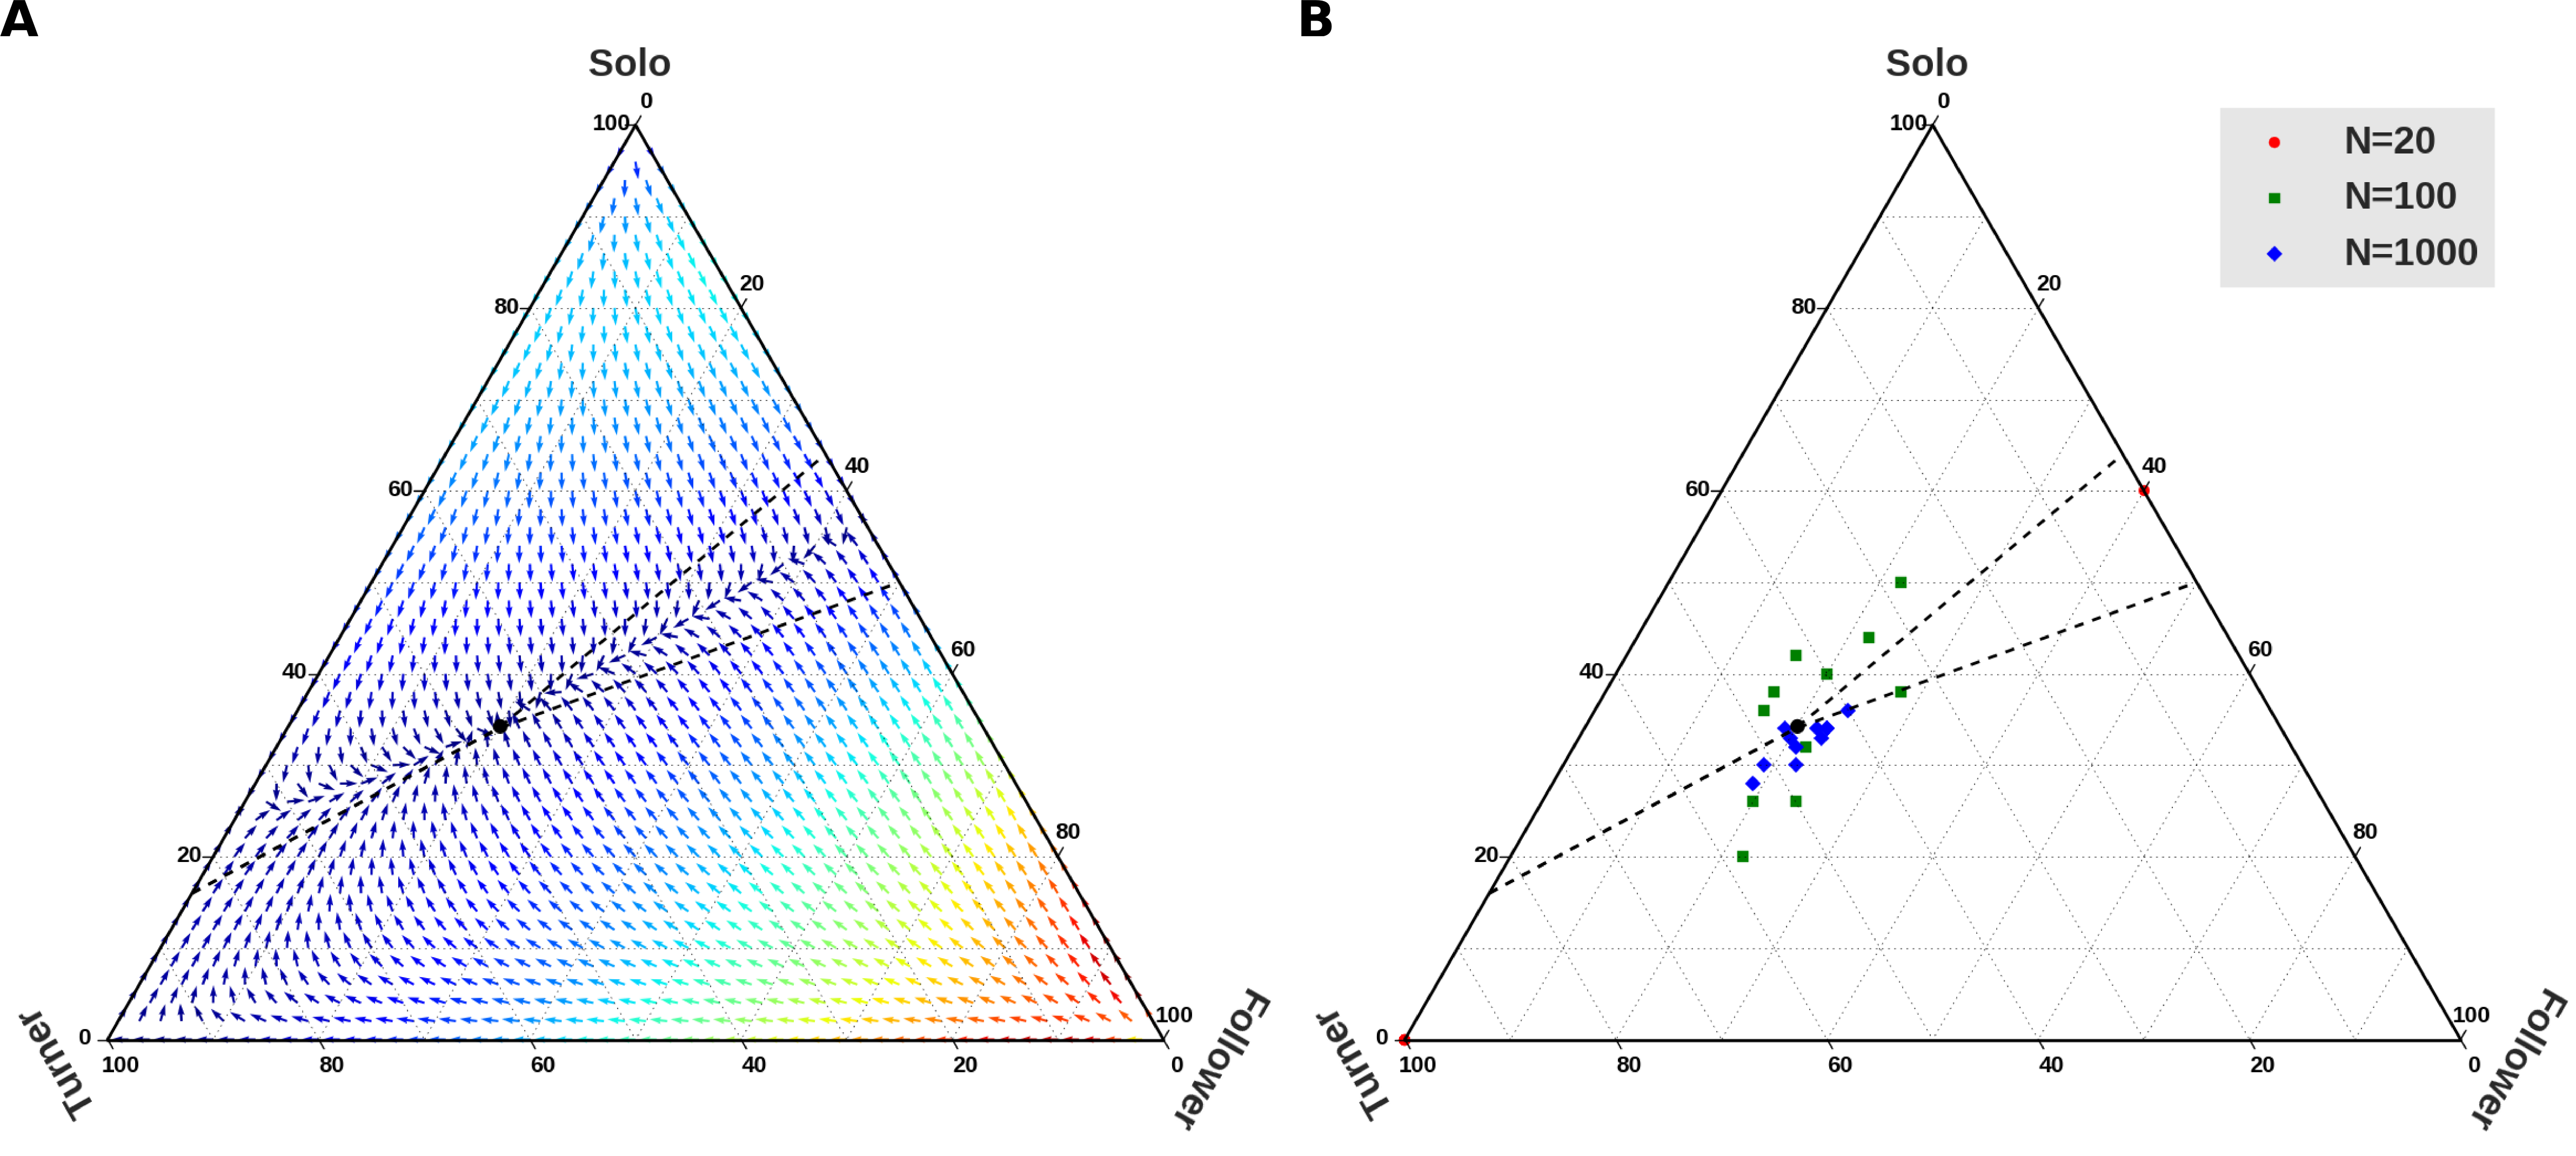
\includegraphics[scale=0.90]{fig/ArticleRob2/figExpectations.png}
    \caption{\textbf{Vector field of the gradient of phenotypes' proportions and proportions of phenotypes at last generation of evolution.} {\em (A)}~Vector field of the gradient of phenotypes' proportions in an infinite population. The strength of variation is indicated by the color of the arrow. {\em (B)}~Repartition of phenotypes at the last generation of evolution for all three population sizes. Evolution lasted $1500$ generations and results were replicated across $11$ independent simulations. The initial population was entirely composed of \emph{leaders}.}
    \label{fig:ternary}
  \end{figure}

  Figure~\ref{fig:ternary}(B) shows the final repartition of phenotypes after $1500$ generations of evolution for \(N=20\), \(N=100\) and \(N=1000\) in $11$ independent replicates. We can see that when increasing population size we also increase the probability that an equilibrium where the three phenotypes exist is reached. We actually observe that the repartition of phenotypes at last generation of evolution gets closer to the predicted equilibrium as population size increases. This implies that when population size increases, the probability to lose particular phenotypes decreases. In other words, the effect that the stochasticity of fitness evaluation has on the sampling of the genotypes for the next generation is mitigated: population size is essential to the maintenance of specialists.


\section{Key Properties for Evolving Heterogeneous Behaviours}
  From the previous Section, we can hypothesize two key properties for the successful evolution of genotypic polymorphism. First, we showed that population size needed to be large enough in order to decrease the probability that heterogeneity could be lost during the evolutionary time. Even under an elitist selection where the best individuals are immediately selected, the stochastic nature of fitness evaluation entails that there is no guarantee that both types get selected. This means that a performance biased selection may lead to the composition of the new population not accurately representing the genotypic diversity of the previous one. Therefore, there needs to be a mechanism for the preservation of genotypic diversity. Second, we previously saw that one key reason for the invasion of \emph{turner} individuals is that, while \emph{followers} perform badly against themselves, this is not the case for the formers. This means that the manner in which robots are paired is essential for achieving specialisation.

  In order to test these hypotheses we design a last experiment where we diverge from the initial problem and now coevolve two separate populations. In this coevolution algorithm, each individual of one population is always evaluated against an individual of the other population ($5$ times as in previous experiments). Then, each population separately undergoes selection under an elitist \((10+10)\) selection method to create the population of the next generation (which means that each population size is $20$). We conducted $11$ independent replicates which lasted $90000$ evaluations each. The populations were initially constituted of random individuals.

  \begin{table}[ht]
    \center{
      \begin{tabular}{cccc}
        \hline
        \textbf{\# L/F} & \textbf{\# Turning} & \textbf{\# NC} & \textbf{Total}\\ 
        \textbf{Strat.} & \textbf{Strat.} & \textbf{Strat.} & \\ 
        \hline
        11 & 0 & 0 & \textbf{11}\\
        \hline
      \end{tabular}
    }
    \caption{\textbf{Strategies evolved by the best individuals when coevolving two populations.} Repartition of the different strategies adopted bt the best individuals at the last evaluation in each of the $11$ replicates. We indicate in each cell the number of simulations where a particular strategy evolved. Two populations were coevolved under elitist selection and the individuals' genotype values were initially random. In the table "L/F" stands for leader/follower and "NC" for "Non-Cooperative".}
    \label{tab:coevoStrategies}
  \end{table}

  We show (Table~\ref{tab:coevoStrategies}) that when using coevolution, we always evolve specialists in every replicates. Moreover, this algorithm is highly stable as the heterogeneous behaviours that emerged were never lost during evolution in every replicates. This means that coevolution is highly efficient both for the bootstrap of a leader/follower strategy and its maintenance throughout evolution. Regarding our hypothesized properties, we can check that the coevolution algorithm respects both of them. Firstly, as populations are separatly coevolved, we make sure that performance-based selection does not accidentally lead to the disappearance of specialists. Thus we ensure that the populations' genotypic diversity is highly protected. Secondly, we create a very specific pairing between individuals. Indeed individuals inside the same population are never partnered with one another. This means that \emph{followers} are always paired with \emph{leaders}. As \emph{turners} thus possesses no fitness benefit over the other phenotypes, their invasion is prevented. The question is open as to how to endow an algorithm working on a single population with such properties.

\section{Discussion and Conclusions}
\label{sec:discussion}
  In this paper, we investigated the evolution of specialisation through a leader/follower strategy in a cooperative foraging task. Our goal was to reveal the difficulties that arise when trying to evolve genotypic polymorphism in a single population. To that end, we mainly studied the dynamics of evolution with two different selection methods: an \((\mu + \lambda)\) elitist evolution strategy and fitness-proportionate selection.

  We first showed that the long term evolution of a leader/follower strategy was nearly impossible with an elitist selection. However bootstrapping specialists was not a problem as we observed that they frequently emerged during evolution. The major obstacle was rather to maintain heterogeneity over evolutionary time. Indeed, even when adding efficient followers to a population of leaders to force the adoption of a leader/follower strategy, specialists couldn't be maintained. In comparison, the properties shown by the fitness-proportionate algorithm were quite the opposite. While it was almost not capable of evolving a leader/follower strategy (nor any other cooperative strategy), the fitness-proportionate selection demonstrated high stability. It was therefore capable of maintaining specialists when present. We thus revealed two critical properties for evolving heterogeneous behaviours in a single population: \emph{bootstrapping} these behaviours and \emph{maintaining} them throughout evolution.

  We then ran computational analyses and showed that while a pair of turners is indeed less efficient w.r.t. payoff than a pair of leader and follower, it is a lot more efficient than a pair of leaders or a pair of followers. As a result, these individuals can easily invade part of the population. Moreoever, we also showed that the maintenance of specialists was very sensible to population size. Performance biased selection can indeed affect heterogeneity in the composition of the next generation's population. Finally, a coevolution algorithm, which we showed to be always successful in evolving heterogeneous behaviours, solved both of these two problems with (1) \emph{specific partners selection} as pairs were constituted of individuals from different populations and (2) \emph{protection} of the behaviours evolved by applying selection separately on the two populations. While this algorithm is not concerned with genotypic polymorphism in a single population, it is useful to yield effective mechanisms which could be studied to solve our problem. 

  This raises several interesting perspectives on how to solve this problem. First, niche protection could prevent the disappearance of the efficient but unstable leader/follower strategy. As a matter of fact, coevolution is akin to a particular type of niches protection with $2$ niches. However, such mechanism could be implemented without specifying the explicit number nor the organization of the niches. Rewarding diversity~\parencite{Lehman2008} is also known as an effective way to protect novel behaviours and could be another promising direction. In particular, a multiobjective algorithm on performance and diversity~\parencite{Doncieux2014}, by rewarding genotypic and phenotypic diversity, may protect evolved specialists.

  Secondly, we showed that because partners were chosen randomly among the population, it created the opportunity for a "parasitic" strategy to invade. An interesting direction for future works could be to investigate restrictions in the choice of partners. For example it would be compelling to investigate how the individuals could evolve to select their partner based on genotypic or phenotypic information.